\documentclass[a4paper]{scrartcl}
\usepackage[
    typ=ueb,
    klausurtyp=kurs,
    klasse=scrartcl,
    fach=LF05 Physik,
    lerngruppe=T20E,
    loesungen=seite,
    module={Symbole,Bewertung}    
    %erwartungshorizontAnzeigen,
    %erwartungshorizontStil=simpel,
hHh]{schule}
% Dieses Dokument gehört zu den Beispiel des LaTeX Paketes Schule und ist von den Autoren
% des Pakets erstellt worden.
%
% Das Dokument steht unter der Lizenz: Creative Commons by-nc-sa Version 4.0
% http://creativecommons.org/licenses/by-nc-sa/4.0/deed.de
%
% Nach dieser Lizenz darf das Dokument beliebig kopiert und bearbeitet werden,
% sofern das Folgeprodukt wiederum unter gleichen Lizenzbedingungen vertrieben
% und auf die ursprünglichen Urheber verwiesen wird.
% Eine kommerzielle Nutzung ist ausdrücklich ausgeschlossen.

\author{Heiko Schröter}
\date{\today}
\title{Bedeutende Physiker\\
(Rechercheaufgabe)}
\subtitle{Übungsaufgaben zur Reflexion und Brechung}

\usepackage{amsmath}
\usepackage{pgfplots}
\usepackage{mathrsfs}
\usepackage{xfrac}
\usepackage{siunitx}
%\sisetup{quotient-mode = fraction, locale = DE}
\sisetup{per-mode = fraction, locale = DE}
\usepackage{blindtext}
\usepackage{enumitem}
\usepackage{longtable}
\newcommand{\Ergebnis}[1]{\underline{\underline{#1}}}

\begin{document}
%\punktuebersicht*

\setzeAufgabentemplate{schule-keinepunkte} 

\begin{aufgabe}[points={6}]
	\begin{itemize}

	\item Recherchieren Sie zum genannten Physiker und stellen Sie den Physiker kurz vor. (Wann geboren, Wo gelebt, Welche bedeutenden Entdeckungen oder Erfindungen ... )
	\item Beschreiben Sie eine Entdeckung oder Erfindung des Physikers genauer.
		
	\end{itemize}
	% \usepackage{array} is required
	\begin{longtable}{|>{\centering\arraybackslash}p{4.2cm}|>{\centering\arraybackslash}p{4.2cm}|>{\centering\arraybackslash}p{4.2cm}|}
	\hline 
	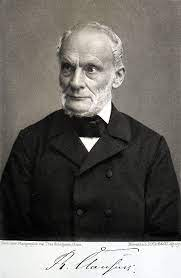
\includegraphics[scale=0.5]{Clausius.jpg} & 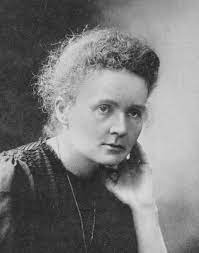
\includegraphics[scale=0.5]{Curie.jpg} & 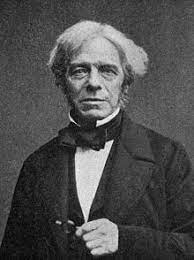
\includegraphics[scale=0.5]{Faraday.jpg} \\ 
	\hline 
	Rudolf Clausius & Marie Curie & Michael Faraday \\ 
	\hline 
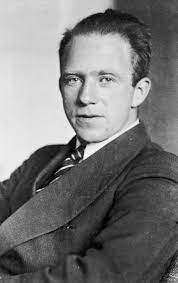
\includegraphics[scale=0.5]{Heisenberg.jpg} & 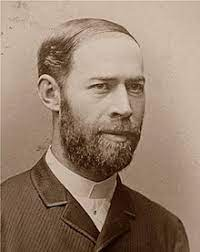
\includegraphics[scale=0.5]{Hertz.jpg} & 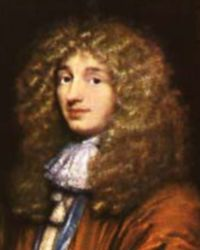
\includegraphics[scale=0.5]{Huygens.jpg} \\
	\hline 
	Werner Heisenberg & Heinrich Hertz & Christiaan Huygens \\ 
	\hline 
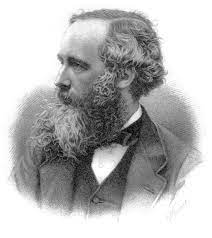
\includegraphics[scale=0.5]{Maxwell.jpg} & 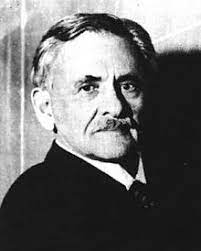
\includegraphics[scale=0.5]{Michelson.jpg} & 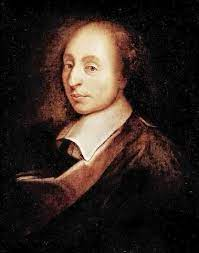
\includegraphics[scale=0.5]{Pascal.jpg} \\
	\hline 
	James Clerk Maxwell & Albert Abraham Michelson & Blaise Pascal \\ 
	\hline 
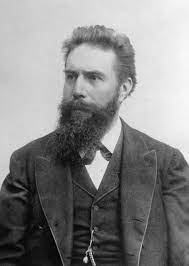
\includegraphics[scale=0.5]{Roentgen.jpg} & 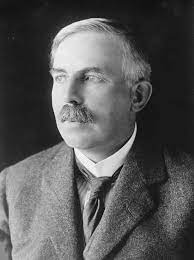
\includegraphics[scale=0.5]{Rutherford.jpg} & \includegraphics[scale=0.5]{Schrödinger.jpg} \\ 
	\hline 
	Wilhelm Conrad Röntgen & Ernest Rutherford & Erwin Schrödinger \\ 
	\hline 
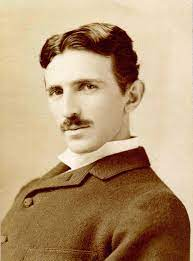
\includegraphics[scale=0.5]{Tesla.jpg} & 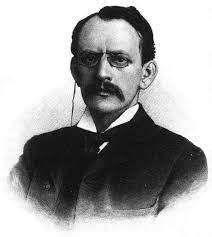
\includegraphics[scale=0.5]{Thomson.jpg} & 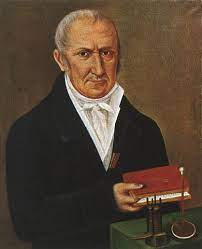
\includegraphics[scale=0.5]{Volta.jpg} \\ 
	\hline 
	Nikola Tesla & Joseph John Thomson & Alessandro Volta \\ 
	\hline 
	\end{longtable}
	
    \begin{loesung}
    keine
    \end{loesung}
\end{aufgabe}
\vspace{0.3cm}

\end{document}